%!TEX root = ../notebook_template.tex
\part{Image Processing}

\section{Norms}

$L_1$ norm

$L_2$ norm

Huber’s norm

$L_\infty $

\section{Computational Photography}

Bayer Pattern

\section{Image Analysis}

\textbf{Hough transform} - line representation - line equation and radial.

\subsection{Integral Images}

The value at any point $(x, y)$ in the summed-area table is the sum of all the pixels above and to the left of (*x*, *y*), inclusive where $i(x,y)$  is the value of the pixel at $(x,y)$. The summed-area table can be computed efficiently in a single pass over the image:

$I(x,y) = i(x-1,y-1) + I(x,y-1) + I(x-1,y)-I(x-1,y-1)$

and similarly for any rectangular region:

$ i(A,B,c,D) = I(D) - I(B) - I(C)+I(A)$

\section{Filtering}

\textbf{Peak Signal To Noise Ratio} 
$max(I)/noise$


\begin{itemize}
\item Color Conversion
\item Thresholding
\item Smoothing
\item Morphology
\item Gradient
\end{itemize}

\subsection{Sobel Operator}
Uses $3\times3$ operators which are convolved with the image to compute approximate (center difference?) derivatives in $x$ and $y$ directions.

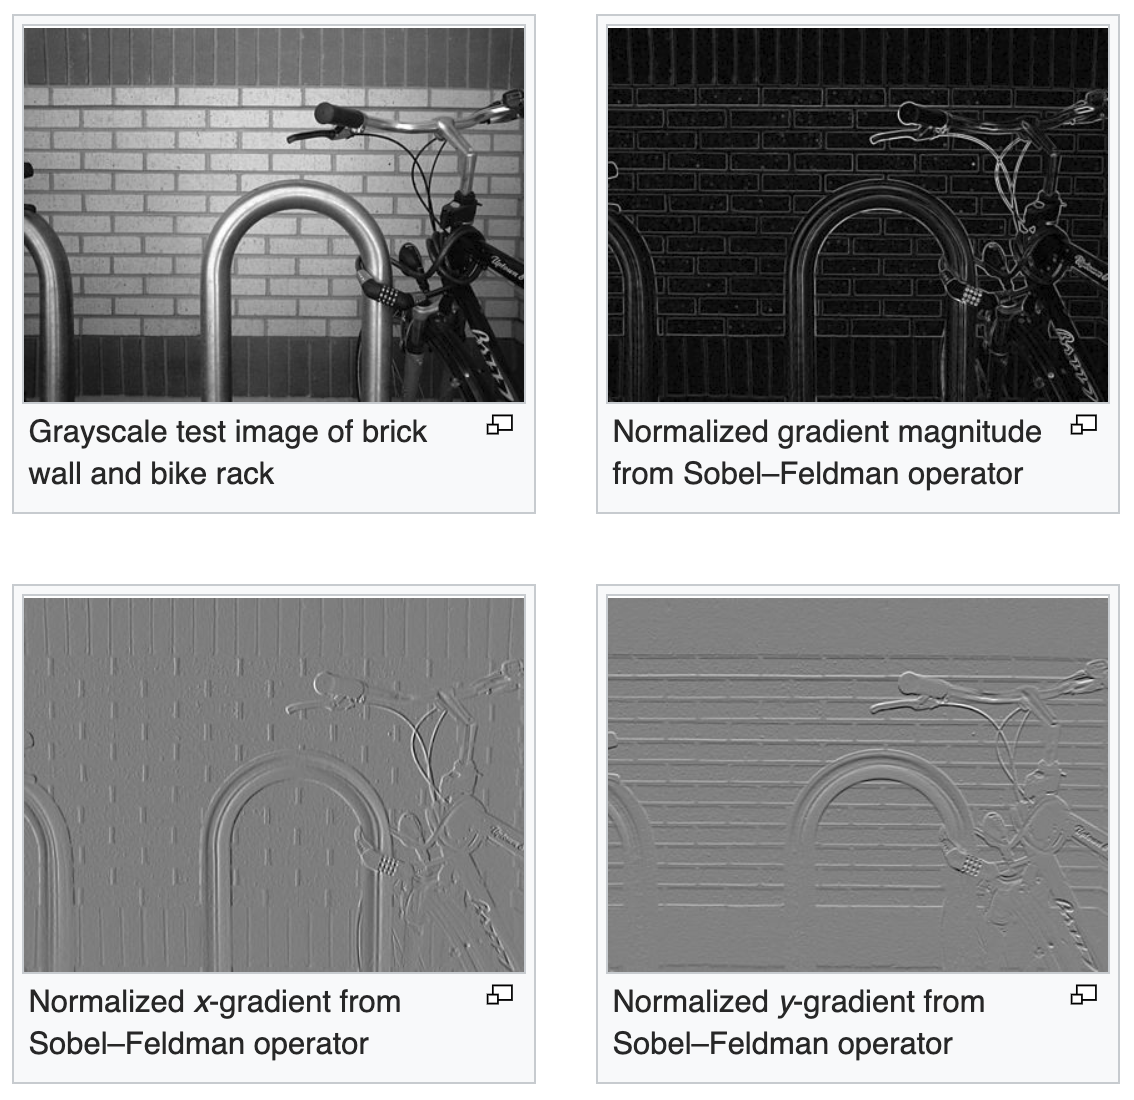
\includegraphics[width=0.9\columnwidth]{sobel.png}
Source: Wikipedia.

\subsection{Canny Edge Detection}
\begin{enumerate}
\item Apply Gaussian filter to smooth the image in order to remove the noise
\item Find the intensity gradients of the image
	The edge orientation is the atan of the intensity of the gradient in each dimension
	The edge magnitude is the sqrt
\item Apply non-maximum suppression to get rid of spurious response to edge detection
\item Apply double threshold to determine potential edges
\item Track edge by hysteresis: Finalize the detection of edges by suppressing all the other edges that are weak and not connected to strong edges.
\end{enumerate}

\textbf{Contours}
\textbf{Histograms}

\subsection{Convolution}

\section{Image Deblurring}

\section{Fourier Transform}

\section{Image Compression}

\section{Optic Flow}

\subsection{Gaussian Pyramids}

Gradient consistency assumption + intensity consistency assumption

Iterative multi scale + warping

Uses an analytic formulation derived from Euler-Lagrange Equations

Results in a dense optic flow field.

Works well for small changes.

\section{Interpolation}


\subsection{Nearest Neighbor}

\subsection{Bilinear Interpolation}

Linear interpolation on a 2D grid. 

\section{De-Convolution and Aliasing}

Band limited filtering

Nyquist Frequency

\section{Noise Models}

\subsubsection{Salt and Pepper / Black White}
This type of noise happens due to sudden interruption in the image signal.
Also known as data drop noise because statistically its drop the original data values
Can be removed using median or morphological filtering.

\subsubsection{Gaussian noise}
Noise which has a probability density function (PDF) equal to that of the normal distribution.
Can be estimated by taking a dark image and measuring the variance of the pixels. Removed by smoothing.


\section{Event Cameras}

\subsection{Features}

\begin{itemize}
\item Low-latency ($\sim1 \mu s$)
\item No motion blur
\item High dynamic range (140 dB instead of 60 dB)
\item Ultra-low power (mean: 1mW vs 1W)
\end{itemize}

Traditional vision algorithms cannot be used because:
\begin{itemize}
\item Asynchronous pixels
\item No intensity information (only binary intensity changes)
\end{itemize}

But they bring new possibilities:
\begin{itemize}
\item Night vision
\item Compact representation and data
\end{itemize}

On static scenes, they mostly produce noise

Main visible features - edges. 

\subsection{Linearized Event Generation}

An event is triggered $\log I(x,t) \log I(xt-\Delta t)=\pm C$

Where $C$ is the minimal contrast which is required for triggering an event, scene dependent.

Consider a pixel $p(x,y)$ with gradient $\nabla L(x,y)$ undergoing a motion $u\in(u,v)$ induced by a moving point $p \in\mathbb{R}^3 $

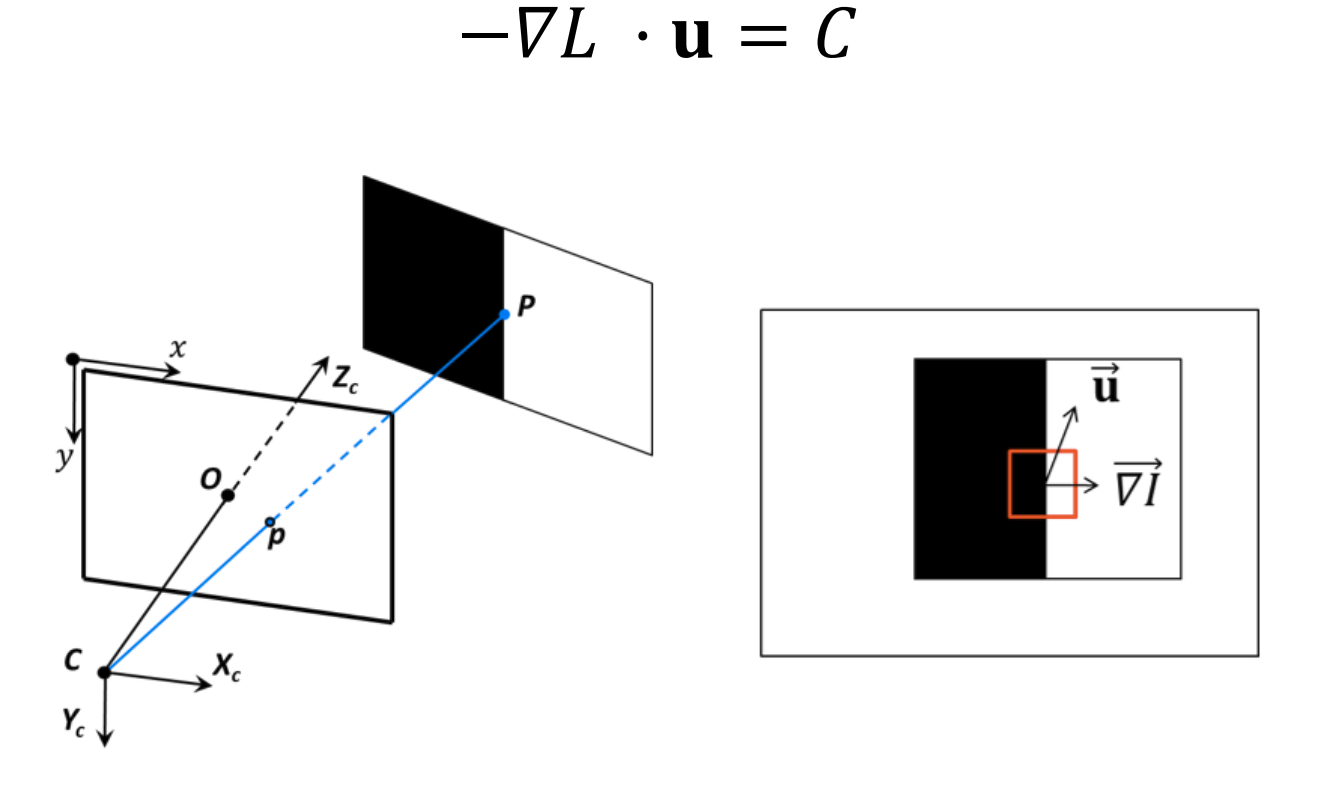
\includegraphics[width=0.9\columnwidth]{event_cameras.png}

Source: State of the Art Report on Event Cameras

From brightness constancy assumption:

$L(x,y,t) = L(x+u,y+v,t+\Delta t)$ from first order approx we get the following $-\nabla L \cdot \vec u = C$

\subsubsection{Deblurring}

A blurry image can be regarded as the integral of a sequence of latent images during the exposure time, while the events indicate the changes between the latent images.

Sharp images are done by subtracting the double integral of the events.

\subsection{(Sparse) Feature Tracking In Event Space}

\subsection{Kanade–Lucas–Tomasi}

Goal: extract features on frames and track them using only events in the blind time between two frames

Uses the event generation model via joint estimation of patch warping and optic flow

Disadvantages: requires GPU for real time tracking and they require knowledge of contract sensitivity, which is scene dependent and differs from pixel to pixel.	

\subsection{Image Reconstruction from Event Cameras}

Recurrent neural network (main module: Unet) 

Input: last reconstructed frame + sequences of event tensors (spatio-temporal 3D voxels grid: each voxel contains sum of ON and OFF events falling within the voxel)

Network processes last $N$ events (10,000) 

Trained in simulation only (without seeing a single real image) (we used our event camera simulator: \url{http://rpg.ifi.uzh.ch/esim.html} Noise free simulation with randomized contrast sensitivity.
